\documentclass[9pt,twocolumn,twoside]{pnas-new}
\setboolean{displaywatermark}{false}

\articletype{SUSTAINABILITY SCIENCE}

\templatetype{pnasresearcharticle}
\graphicspath{{figures/}}
\setkeys{Gin}{draft=false}

\begin{document}

\title{Infrastructure form shapes equitable access to essential services under flooding in Philippine cities}

\author[a]{Noam Anglo}
\author[b]{Eileen Chen}
\author[c]{Sophie Pesek}
\author[d]{Kevin Skinner}
\author[e,1]{Anders Vestrum}

\affil[a]{Development Engineering Program, University of California, Berkeley, Berkeley, CA 94720}
\affil[b]{Department of City and Regional Planning, University of California, Berkeley, Berkeley, CA 94720}
\affil[c]{Energy and Resources Group, University of California, Berkeley, Berkeley, CA 94720}
\affil[d]{School of Information, University of California, Berkeley, Berkeley, CA 94720}
\affil[e]{Department of Electrical Engineering and Computer Sciences, University of California, Berkeley, Berkeley, CA 94720}

\leadauthor{Anglo}

\significancestatement{Flood studies often map where water goes, but communities also lose access when flooded roads sever routes to hospitals, schools, markets, and pharmacies. This study links flood hazard maps, road networks, population grids, and essential-service locations to measure the indirect loss of access across Philippine cities. The framework helps identify neighborhoods that may be isolated outside inundation zones and road segments whose protection would preserve the greatest service access. It offers a reproducible way to translate flood exposure into infrastructure priorities for local planners working under scarce adaptation budgets.}

\authorcontributions{N.A. led project framing and Philippine context; E.C. developed the network, routing, and accessibility methodology; S.P. led environmental and demographic data analysis and figure development; K.S. developed the Reddit corpus and behavioral validation pipeline; A.V. led cross-source flood validation, network-criticality framing, and manuscript integration. All authors contributed to writing and interpretation.}
\authordeclaration{The authors declare no competing interest.}
\correspondingauthor{\textsuperscript{1}Correspondence should be addressed to A.V.}

\keywords{flood resilience $|$ road networks $|$ accessibility $|$ infrastructure equity $|$ Philippines}

\begin{abstract}
Flood risk in cities is usually assessed by overlaying inundation maps with exposed population and assets. That view misses an important mechanism of harm: residents can lose access to essential services when flooded road segments sever routes, even if neither the resident nor the facility is directly flooded. We develop a reproducible network-accessibility framework for ten Philippine cities that combines OpenStreetMap road networks and service locations, LandScan population grids, Project NOAH flood hazard layers, and Google Groundsource historical flood observations. Baseline results show substantial variation in road-network hierarchy, facility coverage, and pre-flood access to hospitals, schools, markets, and pharmacies. Betweenness centrality is highly concentrated in every city, with Gini coefficients between 0.82 and 0.93, indicating that a small set of links can structure a large share of shortest-path flow. Facility data are uneven: schools are broadly represented, while hospitals and pharmacies are sparse in several cities and require quality assurance against official registries. The flood-disruption model removes road edges intersecting medium- or high-depth Project NOAH polygons and recomputes enhanced two-step floating catchment area accessibility to identify direct and indirect access losses. Historical flood observations from Groundsource support NOAH hazard zones while highlighting spatial uncertainty in urban areas such as Manila.
\end{abstract}

\dates{This manuscript was compiled on \today}

\maketitle
\thispagestyle{firststyle}
\ifthenelse{\boolean{shortarticle}}{\ifthenelse{\boolean{singlecolumn}}{\abscontentformatted}{\abscontent}}{}

\Firstpage

\dropcap{F}looding is a central infrastructure and equity challenge for Philippine cities. The Philippines ranked first in the 2025 WorldRiskIndex, and the report's local flood-exposure analysis identifies several Philippine provinces as among the highest-risk subnational areas \cite{worldrisk2025}. PAGASA reports that the Philippine Area of Responsibility receives roughly 20 tropical cyclones per year, with about eight or nine crossing the country \cite{pagasa2026}. Recent evidence also suggests that the frequency of super typhoons in the Philippine Area of Responsibility increased sharply after the late 1990s \cite{basconcillo2025}. These hazards operate through infrastructure systems: roads that fail during floods can fragment cities, delay emergency response, and isolate households from routine services.

Existing work provides pieces of this problem. Global and national flood-network studies show that local inundation can produce nonlocal road-network failure \cite{wang2019,boeingha2024}. City-scale studies have overlaid flood footprints on road graphs to measure topological degradation \cite{casali2019}, while accessibility studies use two-step floating catchment area methods to estimate spatial service availability under ordinary conditions \cite{luo2009,chen2019}. However, many accessibility applications treat networks as static, while many flood-network studies focus on connectivity rather than supply, demand, and competition for services.

We bridge these streams by coupling real flood-hazard footprints with network-routed enhanced two-step floating catchment area (E2SFCA) accessibility. The empirical setting is ten Philippine cities selected from provinces highlighted by the WorldRiskReport local flood-exposure analysis. For each city, we combine OpenStreetMap roads and facilities \cite{boeing2017,openstreetmap}, LandScan 2023 population grids \cite{landscan2023}, and Project NOAH flood hazard layers \cite{lagmay2017,projectnoah}. We use Google Groundsource, an open-access historical flood-event dataset derived from news media, as a complementary check on modeled hazard exposure \cite{google2026}.

The analysis is designed to answer three linked questions. First, how do baseline road-network form and facility geography differ across Philippine cities? Second, where is access to hospitals, schools, markets, and pharmacies already unequal before flooding? Third, when flood hazard is imposed on the road network, which neighborhoods lose access indirectly because surrounding links fail? We report the integrated framework, baseline accessibility, flood-exposure validation, and post-flood analysis design, with final edge-removal estimates reserved for the next computational pass.\par\normalcolwidth

\section*{Results}

\subsection*{Study areas and network structure}
The study sample spans a large urban hierarchy, from Metro Manila's 16.8 million LandScan-estimated residents to Ilagan's 133,000. The corresponding road networks contain 142,178 nodes and 353,725 directed edges across all cities, with Manila accounting for more than half of both nodes and edges (Table \ref{tab:city_networks}; Fig. \ref{fig:study_area}). Average node degree is relatively stable, ranging from 4.63 in Dagupan to 5.34 in Daet, which suggests that local intersection connectivity alone is not a strong differentiator across the sample.

The more important structural variation is hierarchy. Betweenness centrality is concentrated in every city: the betweenness Gini ranges from 0.820 in Daet to 0.931 in Manila. This implies that a small fraction of road nodes mediate a large share of shortest paths. The mechanism differs by urban type. Manila combines dense infrastructure with extreme flow concentration, suggesting potential vulnerability to corridor disruption. Smaller and rural cities show lower hierarchy but greater dependence on dispersed facilities and fewer redundant alternatives.

\begin{table*}[t!]
\centering
\caption{Study-city scale and road-network structure.}
\label{tab:city_networks}
\begin{tabular*}{\textwidth}{@{\extracolsep{\fill}}lrrrrrrr@{}}
City & Population & Nodes & Edges & Avg. deg. & Max BC & BC Gini & Hosp. \\
\midrule
Manila & 16,805,098 & 81,760 & 204,883 & 5.01 & 0.234 & 0.931 & 286 \\
San Fernando & 985,309 & 18,647 & 45,375 & 4.87 & 0.241 & 0.890 & 40 \\
Dagupan & 739,388 & 6,605 & 15,307 & 4.63 & 0.260 & 0.858 & 20 \\
Cagayan de Oro & 729,578 & 11,301 & 27,689 & 4.90 & 0.175 & 0.869 & 13 \\
Cotabato & 523,027 & 3,012 & 7,405 & 4.92 & 0.459 & 0.833 & 10 \\
Naga & 470,868 & 5,852 & 15,238 & 5.21 & 0.258 & 0.845 & 9 \\
Butuan & 347,820 & 5,823 & 14,564 & 5.00 & 0.297 & 0.841 & 12 \\
Tuguegarao & 269,517 & 3,944 & 9,693 & 4.92 & 0.371 & 0.845 & 11 \\
Daet & 152,260 & 2,472 & 6,595 & 5.34 & 0.378 & 0.820 & 7 \\
Ilagan & 133,307 & 2,762 & 6,976 & 5.05 & 0.485 & 0.837 & 2 \\
\bottomrule
\end{tabular*}
\addtabletext{Population is LandScan 2023 population within each study radius. Nodes and edges come from drivable OpenStreetMap graphs retrieved with OSMnx. BC denotes betweenness centrality. Hospital counts are OpenStreetMap points of interest before registry-based quality assurance.}
\end{table*}

\begin{figure}[t!]
\centering
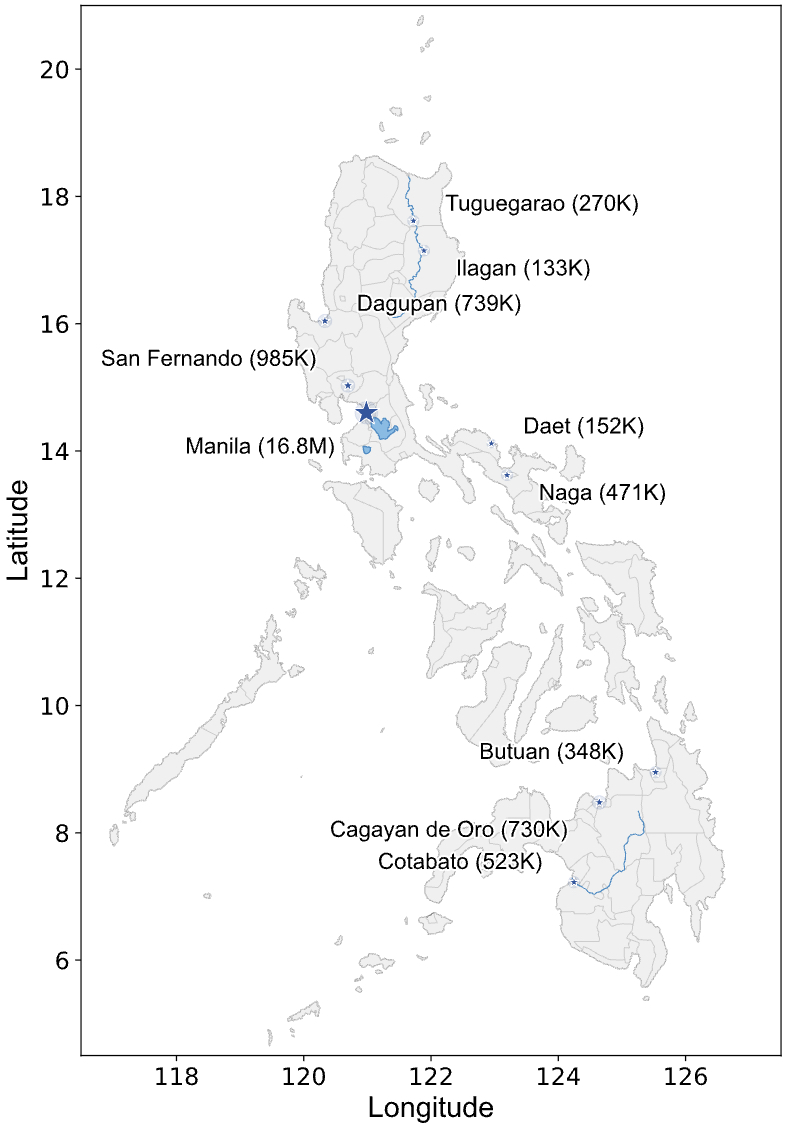
\includegraphics[width=\linewidth]{study_area.png}
\caption{Study cities in the Philippines, labeled by LandScan-estimated population inside each analysis radius. Cities were selected from provinces highlighted as high-exposure areas in the WorldRiskReport local flood-exposure analysis.}
\label{fig:study_area}
\end{figure}

\subsection*{Flood exposure}
Project NOAH 5-year flood hazard polygons show distinct hazard regimes across the ten cities (Fig. \ref{fig:noah_hazard}). Some cities, such as Tuguegarao and Dagupan, display river-corridor patterns in which the major hazard follows a clearly defined floodplain. Others, such as Manila, combine extensive road density with dispersed flood exposure. We use the 5-year return-period scenario because it represents a frequent, planning-relevant hazard rather than a rare catastrophic event. In the post-flood network experiment, roads overlapping medium- or high-depth polygons are removed from the graph; low-depth polygons are retained as passable.

The choice of a medium-depth cutoff is conservative with respect to field evidence from Metro Manila. Mamuyac et al. find that flood depths above 25 cm consistently caused lane closures and reduced vehicle flow by 40--70\% per lane-kilometer as closures increased \cite{mamuyac2025}. Project NOAH categories are categorical rather than continuous, so the analysis treats the medium class (0.5--1.5 m) as the first reliably impassable category and retains the low class (0--0.5 m) for sensitivity testing.

\begin{figure*}[t!]
\centering
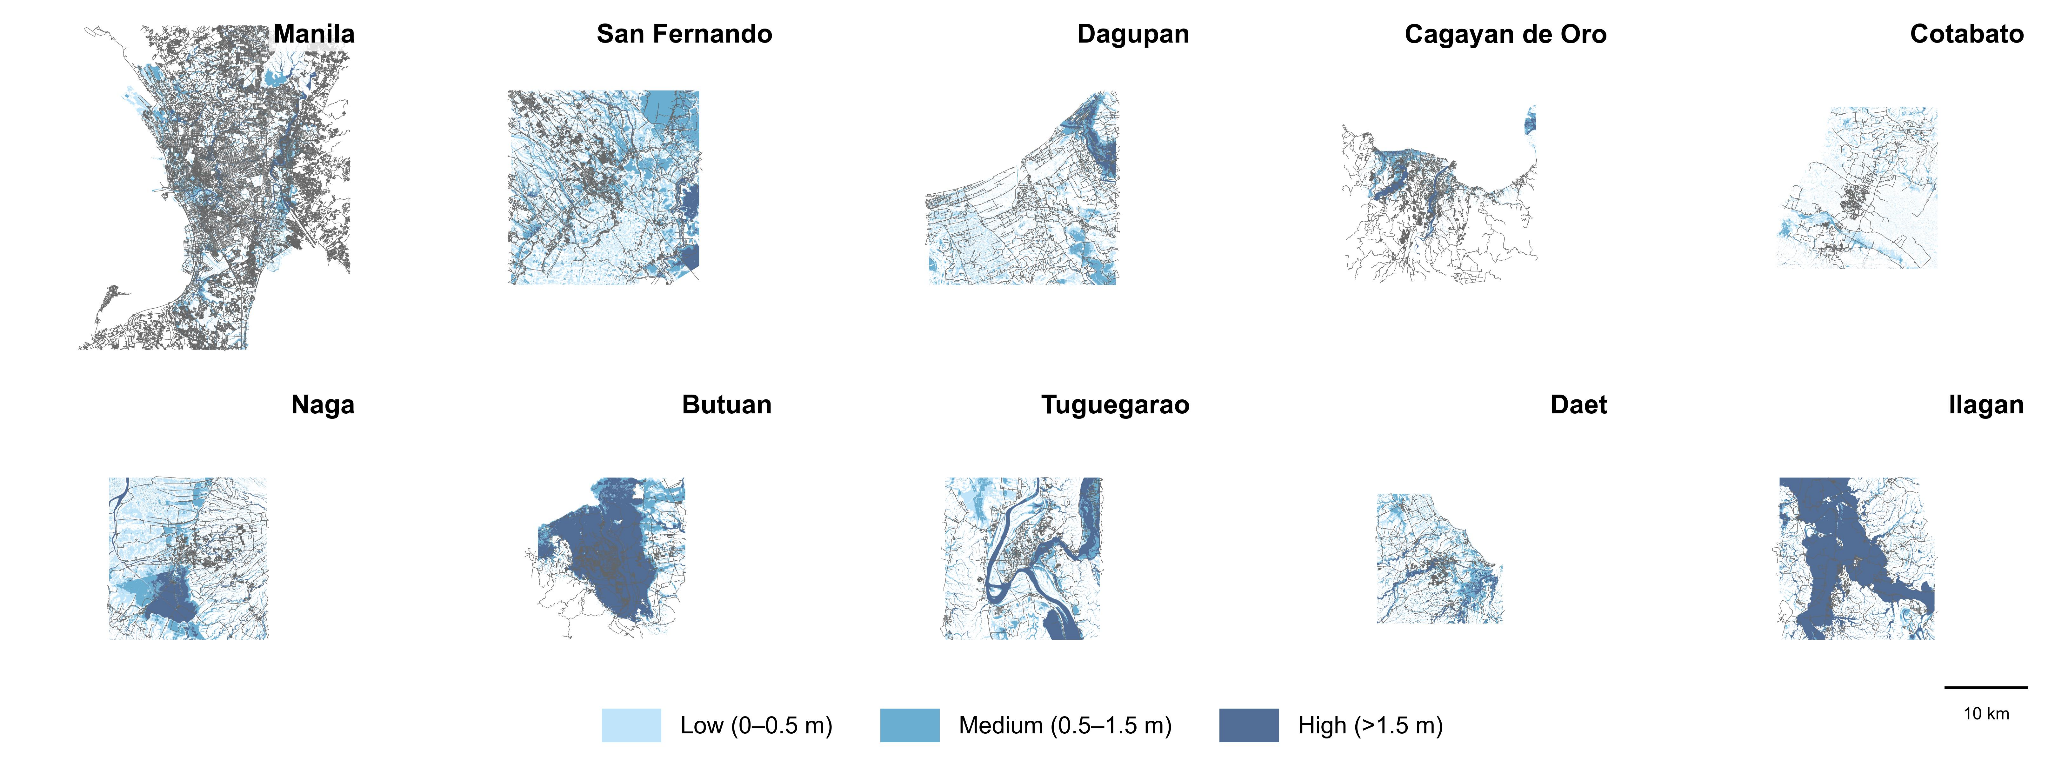
\includegraphics[width=\textwidth]{noah_hazard.png}
\caption{Project NOAH 5-year flood hazard exposure by city. Light, medium, and dark blue represent low (0--0.5 m), medium (0.5--1.5 m), and high ($>$1.5 m) hazard classes. The edge-removal scenario treats medium and high polygons as disruptive to road travel.}
\label{fig:noah_hazard}
\end{figure*}

\subsection*{Facility coverage and baseline access}
OpenStreetMap facility coverage is uneven across service types. Schools are present in meaningful numbers in all cities, while hospitals and pharmacies are sparse in several cases. Ilagan has only two mapped hospitals and one mapped pharmacy, and Cotabato has ten hospitals and fourteen pharmacies. These counts almost certainly reflect a mix of real service scarcity and incomplete tagging. The final facility layer should therefore compare OSM records against Department of Health, Department of Education, and Department of Trade and Industry registries, geocode missing facilities, and deduplicate records within 100 m before policy interpretation.

Baseline E2SFCA scores reveal a stable hierarchy across facility types. Schools have the highest accessibility because they are numerous; hospitals have the lowest because they are fewer and more spatially concentrated. The spatial distribution of hospital access shows the clearest equity stakes (Fig. \ref{fig:hospital_access}). Dense cities such as Manila, Dagupan, and San Fernando maintain relatively high hospital accessibility across much of the urban extent, while several mid-size and smaller cities show core-periphery gradients. Tuguegarao and Ilagan have peripheral cells with very low or zero baseline hospital accessibility before any flood disruption is imposed.

\begin{figure*}[t!]
\centering
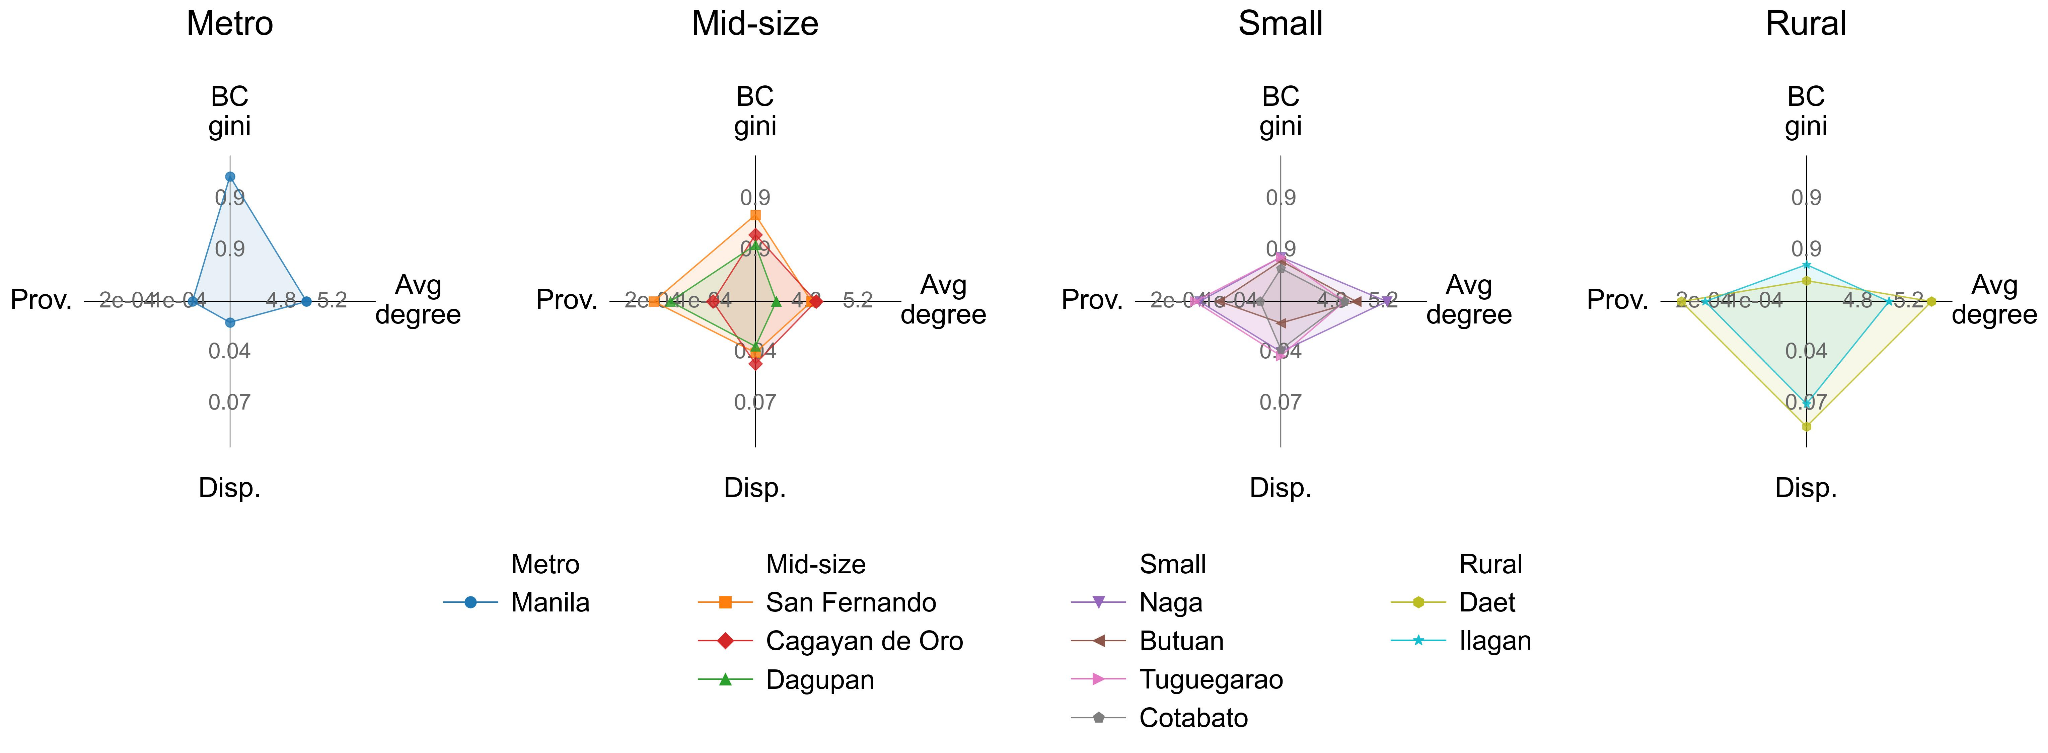
\includegraphics[width=\textwidth]{structural_profiles.png}
\caption{Pre-flood structural vulnerability profiles by city group. Axes summarize betweenness-centrality concentration (BC Gini), average degree, facility provision, and facility dispersion. Manila's profile is dominated by high hierarchy, while smaller and rural cities tend to express vulnerability through facility dispersion and sparse service alternatives.}
\label{fig:structural_profiles}
\end{figure*}

\begin{figure*}[t!]
\centering
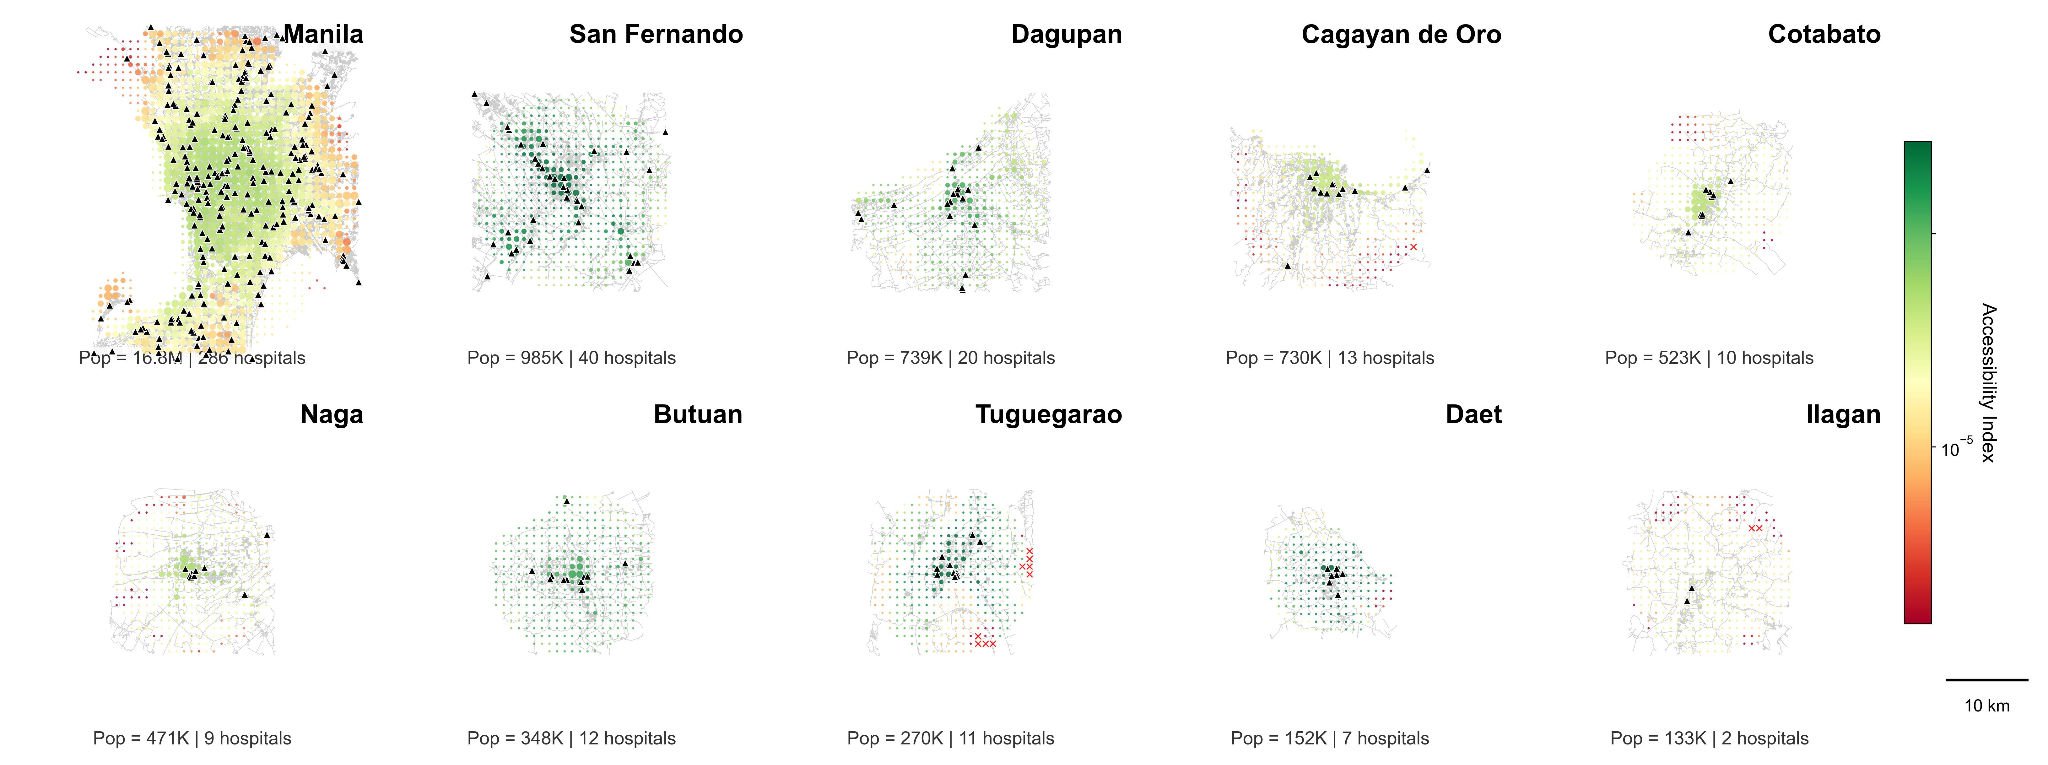
\includegraphics[width=\textwidth]{hospital_access.png}
\caption{Baseline hospital accessibility by city. Colored LandScan demand cells show the E2SFCA accessibility index; black triangles mark OpenStreetMap hospitals; red crosses mark cells with zero reachable hospital access within the 30-minute catchment. These baseline gaps define the reference surface for post-flood access-loss estimates.}
\label{fig:hospital_access}
\end{figure*}

\subsection*{Cross-source flood validation}
Groundsource provides a useful but imperfect empirical check on NOAH hazard exposure. It contains historical flood-event polygons derived from news media, so it is not an inundation map and should not be used to infer precise water depth. Instead, we aggregate Groundsource events from 2001 to 2026 within each study radius and compare the cumulative footprint with the NOAH 5-year hazard layer.

Across the inspected cities, recall is high: most NOAH hazard areas are supported by at least one Groundsource flood observation (Fig. \ref{fig:groundsource}). The overlap is much lower by Jaccard index because Groundsource polygons are often administrative units that are much larger than the actual inundated area. This pattern is especially strong in Manila, where media density and administrative polygon size inflate the Groundsource footprint. The validation therefore supports using NOAH as the primary hazard layer while cautioning against treating either source as exact ground truth.

\begin{figure*}[t!]
\centering
\includegraphics[width=.78\textwidth]{groundsource_validation.png}
\caption{Comparison between Project NOAH 5-year flood hazard and cumulative Google Groundsource flood observations for Tuguegarao, Dagupan, and Manila. High recall indicates that most NOAH hazard areas have historical flood evidence in Groundsource; lower Jaccard values mainly reflect the coarser spatial units used by Groundsource and the aggregation of events over 2001--2026.}
\label{fig:groundsource}
\end{figure*}

\section*{Discussion}

The baseline results suggest that flood vulnerability is not reducible to flood exposure alone. Network form, service distribution, and population geography jointly shape who can reach essential services before and after flooding. Manila's risk is partly a problem of hierarchy: the road network is dense, but shortest-path flow is strongly concentrated. Smaller cities express a different vulnerability: lower facility counts, wider facility dispersion, and more peripheral demand cells near the edge of the 30-minute catchment.

This distinction matters for policy. If flood planning only maps inundated places, it can miss households outside flood polygons that become isolated because connecting roads fail. A network-accessibility view instead identifies road segments whose protection would preserve service access for many residents, including residents who are not directly inundated. These segments are strong candidates for drainage improvements, elevation, emergency-routing protection, or targeted maintenance before recurring seasonal floods.

The main limitation is that the post-flood network simulation is still being finalized. The next computational pass should report, for every city and service type, the share of population losing more than 50\% of baseline access, the share newly disconnected, and the indirect-loss ratio among residents outside the flood zone. Those outputs will allow the structural profiles in Fig. \ref{fig:structural_profiles} to be tested directly against modeled access losses.

\begin{table}[t!]
\centering
\caption{Core modeling parameters.}
\label{tab:parameters}
\begin{tabular}{ll}
Parameter & Value \\
\midrule
Travel-time threshold & 30 min \\
Decay weights & 1.00 / 0.68 / 0.22 \\
Sub-zone boundaries & 10 / 20 / 30 min \\
Facility capacity & 1 per facility \\
Flood removal threshold & NOAH Var $\geq$ 2 \\
Dispersion reference speed & 30 km/h \\
BC sample size & min(300, $|V|$) \\
Network representation & Undirected \\
Demand unit & LandScan cell \\
\bottomrule
\end{tabular} \\
\addtabletext{The NOAH Var $\geq$ 2 threshold corresponds to the medium and high categorical hazard classes. Low-depth polygons are retained as passable in the main specification and reserved for sensitivity testing.}
\end{table}

\matmethods{
\subsection*{Study sample and data sources}
The analysis uses ten Philippine cities selected from provinces highlighted in the WorldRiskReport 2025 local flood-exposure analysis. City radii range from 8 to 20 km and are centered on each city. Road networks and points of interest are extracted from OpenStreetMap using OSMnx \cite{boeing2017,openstreetmap}. Population demand comes from LandScan Global 2023, an ambient population raster at approximately 1-km resolution \cite{landscan2023}. Flood hazard comes from Project NOAH 5-year return-period flood polygons \cite{lagmay2017,projectnoah}. Google Groundsource is used only as a validation layer, not as an edge-removal layer \cite{google2026}.

\subsection*{Road networks and facilities}
Drivable OSM networks are downloaded by city center and radius. OSMnx imputes free-flow speed from \texttt{maxspeed} tags and highway-type defaults, then computes travel time for each edge as $\tau_e = \ell_e/v_e$. Directed graphs are converted to undirected graphs for E2SFCA routing because catchment membership assumes symmetric travel time. Essential-service facilities are extracted for four categories: hospitals (\texttt{amenity=hospital}), schools (\texttt{amenity=school}), markets (\texttt{shop=supermarket} or \texttt{amenity=marketplace}), and pharmacies (\texttt{amenity=pharmacy}). Polygon features are represented by centroids. Each facility is snapped to the nearest graph node with a KD-tree.

\subsection*{Population demand}
LandScan cells are clipped to each city radius, and zero-population cells are dropped. Each remaining cell centroid is snapped to its nearest graph node with the same KD-tree procedure used for facilities. Population is retained at the cell level rather than aggregated to proxy nodes. Multiple cells may share a proxy node, but each cell retains its own population weight.

\subsection*{Enhanced two-step floating catchment area}
For each facility $j$, the weighted population competing for it within the travel-time threshold $d_0$ is
\[
D_j=\sum_{i:\tau_{ij}\leq d_0}W(\tau_{ij})P_i,
\]
where $P_i$ is the population of demand cell $i$, $\tau_{ij}$ is network travel time from cell $i$ to facility $j$, and $W(\cdot)$ is a step-wise distance-decay function. With equal facility capacity $S_j=1$, the supply-to-demand ratio is $R_j=1/D_j$. Cell-level accessibility is then
\[
A_i=\sum_{j:\tau_{ij}\leq d_0}W(\tau_{ij})R_j.
\]
The catchment threshold is 30 min, divided into 0--10, 10--20, and 20--30 min sub-zones with weights 1.00, 0.68, and 0.22 following the slow-decay E2SFCA scheme \cite{luo2009}. Under equal capacity, the population-weighted mean accessibility for a city-service pair equals the service's per-capita provision, which is used as a computational check.

\subsection*{Network structural metrics}
Average degree is computed as $\bar{k}=2|E|/|V|$ on the undirected graph. Betweenness centrality is approximated with $k=\min(300,|V|)$ sampled source nodes and seed 42. The betweenness Gini coefficient is computed from sorted betweenness values $b_1\leq\cdots\leq b_n$ as
\[
G_{BC}=\frac{2\sum_{i=1}^{n}ib_i}{n\sum_{i=1}^{n}b_i}-\frac{n+1}{n}.
\]
Facility provision is the raw count of facilities per capita. Facility dispersion is the median nearest-neighbor network travel time among same-type facilities, normalized by the travel time implied by the city radius and a 30 km/h reference speed.

\subsection*{Flood disruption analysis}
Road edges are spatially joined to NOAH flood polygons. In the main scenario, an edge is removed when its maximum overlapping hazard class satisfies Var $\geq$ 2, corresponding to medium or high modeled depth. E2SFCA is rerun on the degraded graph to produce $A_i^{\mathrm{post}}$. The relative cell-level change is
\[
\delta_i=\frac{A_i^{\mathrm{post}}-A_i^{\mathrm{base}}}{A_i^{\mathrm{base}}}.
\]
City-level summaries will report the population share with severe access loss ($\delta_i < -0.5$) and the share newly disconnected ($A_i^{\mathrm{base}}>0$ and $A_i^{\mathrm{post}}=0$). Affected cells are classified as direct if the cell lies within a flood polygon and indirect if the cell lies outside all flood polygons but loses access because network routes are severed elsewhere. The indirect ratio is the affected outside-flood-zone population divided by total affected population.

\subsection*{Implementation}
Because the routing graph is undirected, both E2SFCA passes are computed from demand-node Dijkstra queries. Dijkstra searches use a sparse adjacency matrix with a 1,800-second cutoff. Demand cells sharing a proxy node are deduplicated during routing and then expanded back to cell-level scores. Cities are parallelized across workers. The Reddit and DHS analyses remain ancillary validation and equity-context modules: the Reddit corpus is used to search for behavioral evidence of mobility disruption, while DHS cluster overlap is reserved for cities with sufficient survey density.
}

\showmatmethods{}

\dataavail{All primary input datasets are publicly available from OpenStreetMap, LandScan Global 2023, Project NOAH or LiPAD hazard-map repositories, Google Groundsource, and the DHS Program subject to each provider's access terms. Analysis code, processed tables, and derived figures should be deposited in a public repository before submission; repository details will be inserted once the final pipeline is frozen.}

\acknow{We thank Professor Joshua Blumenstock for feedback and the students of INFO 288 for comments and encouragement. We also thank members of the University of the Philippines Resilience Institute and Project NOAH community for the scientific data infrastructure that makes this analysis possible.}

\showacknow{}

\bibsplit[9]
\bibliography{pnas-sample}

\end{document}
